\qrchapter{https://forgottenpillar.com/rsc/pl-fp-chapter2}{Fundamentalne zasady}

Prawdziwym problemem, według rozdziału dziesiątego \textit{Special Testimonies}, jest odejście od fundamentu naszej wiary, który został ustanowiony na początku naszego dzieła.

\egw{\textbf{Ten fundament został zbudowany przez Mistrza} i \underline{przetrwa} burzę i nawałnicę. Czy pozwolą temu człowiekowi \textbf{przedstawiać doktryny, które zaprzeczają doświadczeniom z przeszłości} ludu Bożego? Nadszedł czas, aby podjąć zdecydowane działanie}[SpTB02 54.2; 1904][https://egwwritings.org/read?panels=p417.276]

Kellogg przedstawił doktryny, które zaprzeczają doświadczeniom z przeszłości. W innym miejscu napisała o Kelloggu:

\egw{Bardzo martwię się o dr. Kellogga. Pod wieloma względami jego postępowanie nie podoba się Panu. Wydaje się, że \textbf{tak łatwo jest mu odejść od \underline{fundamentalnych zasad}}. Jest w wielkim niebezpieczeństwie, że \textbf{nie zachowa swoich początkowych przekonań} aż do końca}[Lt138-1902.5; 1902][https://egwwritings.org/read?panels=p9219.11]

Problemem było odejście od fundamentalnych zasad — ale nie wszyscy ludzie to dostrzegli. Szczególnie kluczowi i znaczący ludzie w dziele zapomnieli drogę, którą Pan ich prowadził, oraz Jego nauki w przeszłości.

\egw{Miałam nadzieję, że nastąpi gruntowna reforma i że \textbf{zasady}, o które walczyliśmy \textbf{we wczesnych dniach} i które zostały wprowadzone w mocy Ducha Świętego, \textbf{będą zachowane}}[SpTB02 56.3; 1904][https://egwwritings.org/read?panels=p417.287]

Jakie były zasady, o które walczyliśmy we wczesnych dniach? Co było tym fundamentem naszej wiary?

\egw{Jako lud mamy \textbf{stać niewzruszenie na platformie wiecznej prawdy}, która przetrwała próby i doświadczenia. Mamy \textbf{trzymać się pewnych filarów naszej wiary}. \textbf{\underline{Zasady prawdy}}, które Bóg nam objawił, \textbf{są naszym jedynym prawdziwym fundamentem}. To one uczyniły nas tym, czym jesteśmy}[SpTB02 51.2; 1904][https://egwwritings.org/read?panels=p417.261]

\egwinline{Zasady prawdy}, które Bóg objawił, \egwinline{są naszym jedynym prawdziwym fundamentem}. Nazywa ona te zasady platformą wiecznej prawdy. Odnosi się do tych zasad jako do \egwinline{pewnych filarów naszej wiary}[SpTB02 51.2; 1904][https://egwwritings.org/read?panels=p417.261].

Przypomina ona o wcześniejszych doświadczeniach naszych pionierów, takich jak James White, Joseph Bates, starszy Edson, ojciec Pierce, jak Bóg pracował nad nimi, aż \egwinline{punkt po punkcie} \egwinline{wszystkie \textbf{główne punkty naszej wiary} zostały wyjaśnione}. Przypomniała, jak \egwinline{ten fundament został zbudowany przez Mistrza}, i zapewnia, że \egwinline{przetrwa burzę i nawałnicę}. Podsumowując, zdecydowanie potwierdziła wolę Boga wobec nas w kontekście tych zasad. Bóg \egwinline{wzywa nas, abyśmy trzymali się mocno, z uściskiem wiary, \textbf{fundamentalnych zasad}, które są oparte na niepodważalnym autorytecie}.

Widzimy kilka różnych wyrażeń, których siostra White użyła w odniesieniu do fundamentu naszej wiary: „\textit{platforma wiecznej prawdy}”, „\textit{filary naszej wiary}”, „\textit{zasady prawdy}”, „\textit{główne punkty}”, „\textit{drogowskazy}” i „\textit{fundamentalne zasady}”. Wyrażenia te oznaczają to samo — \textit{fundament naszej wiary}. Kiedy dziś słyszymy te określenia, jakoś nie przekazują one żadnych konkretnych informacji. Ale dla Adwentystów Dnia Siódmego w jej czasach było to bardzo jasne i konkretne. Wszystkie te terminy odnoszą się do publicznego streszczenia wiary Adwentystów Dnia Siódmego, zwanego \emcap{Fundamentalnymi Zasadami}, wyjaśnionymi poniżej.

Bóg \egwinline{wzywa nas, abyśmy \textbf{trzymali się mocno}, z uściskiem wiary, \textbf{\underline{fundamentalnych zasad}}, które \textbf{są oparte na niepodważalnym autorytecie}}. Jest to odniesienie do głównych aspektów wiary Adwentystów Dnia Siódmego, które Bóg objawił pionierom adwentyzmu \egwinline{po upływie czasu w 1844 roku}, gdy grupa gorliwych, szlachetnych i prawych mężczyzn \egwinline{poszukiwała prawdy jak ukrytego skarbu}. To był \textit{fundament naszej wiary}. Nasi pionierzy oficjalnie założyli Kościół Adwentystów Dnia Siódmego w 1863 roku i nauczali tych prawd, które nazwali „\textit{fundamentalnymi zasadami}”. Jednak często Adwentyści Dnia Siódmego byli publicznie przedstawiani w niewłaściwy sposób. Z tego powodu w 1872 roku nasi pionierzy opublikowali dokument zatytułowany „\textit{Deklaracja Fundamentalnych Zasad, nauczanych i przestrzeganych przez Adwentystów Dnia Siódmego}” w celu publicznego i zwięzłego zadeklarowania, jakich \emcap{Fundamentalnych Zasad} nauczali i przestrzegali Adwentyści Dnia Siódmego. Te \emcap{Fundamentalne Zasady} były regularnie drukowane jako osobna broszura, były obecne w naszych czasopismach i były corocznie drukowane w Rocznikach Adwentystycznych przez całe życie Ellen White\footnote{Patrz \hyperref[appendix:timeline]{Fundamentalne Zasady — oś czasu}, aby uzyskać więcej szczegółów.}. Dlatego gdy Ellen White odnosiła się do „\textit{fundamentalnych zasad}”, nie było to mgliste czy niejasne stwierdzenie, ponieważ Kościół Adwentystów Dnia Siódmego oficjalnie i publicznie zadeklarował, czym były te \emcap{Fundamentalne Zasady}. We wstępie do tego dokumentu czytamy o celu, który temu dokumentowi przyświecał.

\begin{figure}
    \centering
    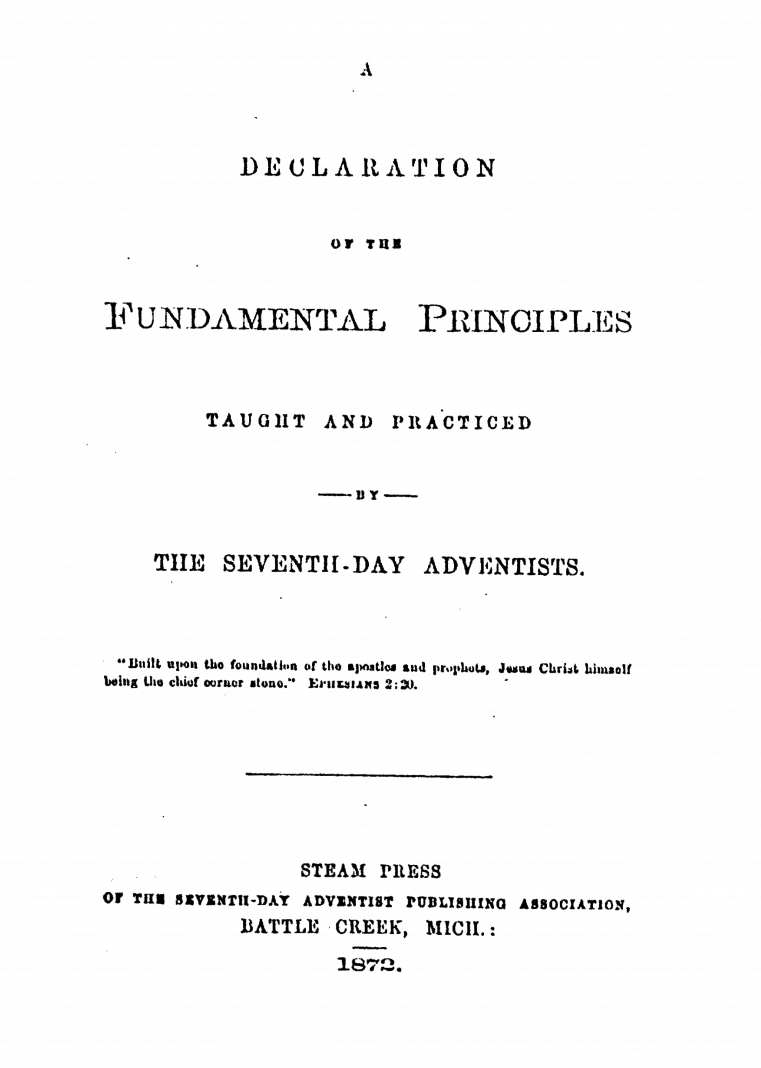
\includegraphics[width=1\linewidth]{images/declaration-of-the-fundamental-principles.PNG}
    \caption*{Skan Deklaracji Fundamentalnych Zasad, 1872.}
    \label{fig:declaration-of-the-fundamental-principles}
\end{figure}

\others{Przedstawiając \textbf{publicznie} to \textbf{streszczenie naszej wiary}, pragniemy, aby wyraźnie zrozumiano, że \textbf{nie mamy żadnych artykułów wiary, wyznania wiary ani dyscypliny} \textbf{\underline{poza Biblią}}. \textbf{Nie} przedstawiamy tego \textbf{jako coś, co ma jakikolwiek autorytet wśród naszych ludzi}, \textbf{ani nie ma to na celu zapewnienia jednolitości wśród nich}, \textbf{jako system wiary}, \textbf{ale jest to krótkie oświadczenie o tym, \underline{co jest i było, z wielką jednomyślnością, wyznawane przez nich}}. Często jest konieczne, aby odpowiadać na pytania dotyczące tego tematu, a czasami korygować fałszywe stwierdzenia rozpowszechniane przeciwko nam i usuwać błędne wrażenia, które powstały u tych, którzy nie mieli okazji zapoznać się z naszą wiarą i praktyką. Naszym jedynym celem jest sprostanie tej potrzebie}

\othersnodotnogap{\textbf{Jako Adwentyści Dnia Siódmego pragniemy jedynie, aby nasze stanowisko było zrozumiane}; tym bardziej nam na tym zależy, ponieważ jest wielu, którzy nazywają siebie adwentystami, a głoszą poglądy, z którymi nie możemy się zgodzić, z których niektóre, jak sądzimy, podważają najprostsze i najważniejsze zasady przedstawione w Słowie Bożym}[Fundamentalne Zasady, 1872, s. 3, akap. 1--2.][https://egwwritings.org/read?panels=p928.8].

To streszczenie wiary składało się z 25 punktów, które reprezentowały to, co \othersnodot{jest i było, z wielką jednomyślnością, wyznawane przez} Adwentystów Dnia Siódmego. Te 25 punktów stanowiło \egwinline{\textbf{fundament}, który został \textbf{położony na początku} naszego dzieła \textbf{poprzez pełne modlitwy studium} Słowa i przez objawienie}. W 1904 roku siostra White powiedziała nam, że \egwinline{na \textbf{tym fundamencie} budujemy przez \textbf{ostatnie pięćdziesiąt lat}}. To są \egwinline{\textbf{fundamentalne zasady, które są oparte na niepodważalnym autorytecie}}, których Bóg \egwinline{wzywa nas, abyśmy \textbf{trzymali się mocno}, z uściskiem wiary}. Innymi słowy, powtórzyła, że \egwinline{mamy \textbf{trzymać się pewnych filarów naszej wiary}}.

W 1904 roku siostra White pisała o \egwinline{\textbf{staraniach wroga, aby podkopać fundament naszej wiary}}. Pisała o ruchu, który miałby \egwinline{polegać na \textbf{porzuceniu} doktryn, które stoją jako \textbf{filary naszej wiary}}. Ta reforma, gdyby została przyjęta, odrzuciłaby \egwinline{\textbf{zasady prawdy}, które Bóg w swojej mądrości dał Kościołowi ostatków}, i \egwinline{\textbf{fundamentalne zasady}, które podtrzymywały dzieło przez ostatnie pięćdziesiąt lat, \textbf{zostałyby uznane za błąd}}. Ruch ten rozpoczął się mniej więcej w czasie, gdy dr John H. Kellogg opublikował książkę \textit{The Living Temple}\footnote{Pl. \textit{Żyjąca Świątynia} (przyp. tłum.).}.

\egw{Mniej więcej w czasie, gdy opublikowano «The Living Temple», w porze nocnej przeszły przede mną \textbf{obrazy wskazujące, że zbliża się jakieś niebezpieczeństwo}, i że muszę się na nie przygotować poprzez  \textbf{spisanie rzeczy}, które Bóg mi objawił \textbf{odnośnie do \underline{fundamentalnych zasad naszej wiary}}}[SpTB02 52.3; 1904][https://egwwritings.org/read?panels=p417.267]

Przez opublikowanie książki \textit{The Living Temple} \textbf{fundamentalne zasady naszej wiary} \textbf{miały być podważone} \egwinline{poprzez rozpowszechnianie \textbf{zwodniczych teorii}} w niej zawartych.

\egw{Zostałam pouczona przez niebiańskiego posłańca, że część rozumowania w książce «The Living Temple» jest niepoprawna i że \textbf{to rozumowanie sprowadziłoby na manowce} umysły tych, którzy nie są całkowicie utwierdzeni w \textbf{fundamentalnych zasadach} teraźniejszej prawdy. Wprowadza to, co jest niczym innym jak spekulacją w \textbf{odniesieniu do \underline{osobowości Boga i tego, gdzie jest Jego obecność}}}[SpTB02 51.3; 1904][https://egwwritings.org/read?panels=p417.262]

Siostra White zwraca szczególną uwagę na to, że rozumowanie zawarte w książce \textit{The Living Temple} \egwinline{\textbf{sprowadziłoby na manowce}} z \egwinline{\textbf{fundamentalnych zasad} teraźniejszej prawdy}. To rozumowanie dotyczy \egwinline{\textbf{osobowości Boga i tego, gdzie jest Jego obecność}}.

Jak wspomniano wcześniej, słowo ‘\textit{osobowość}’ w kontekście dziewiętnastego wieku jest definiowane jako „\textit{właściwość lub stan bycia osobą}”\footnote{„Personality”, „słownik Merriam-Webster” [online], \href{https://www.merriam-webster.com/dictionary/personality}{merriam-webster.com/dictionary/personality} [dostęp: 19 maja 2025].}. Innymi słowy, termin ten odpowiada na pytania: „\textit{Co definiuje kogoś jako osobę?}”, „\textit{Jaka jest właściwość lub stan kogoś jako osoby?}”. W przypadku \emcap{osobowości Boga} pytanie brzmi: „\textit{Czy Bóg jest osobą i co definiuje Go jako osobę? Jaka jest właściwość lub stan Boga jako osoby?}”.

Rozumowanie dr. Kellogga dotyczące tych kwestii, wyrażone w książce \textit{The Living Temple}, jest \egwinline{niepoprawne}. Poglądy dotyczące \egwinline{\textbf{osobowości Boga i tego, gdzie jest Jego obecność}}, \egwinline{propagowane w książce, nie miały poparcia Boga i były \textbf{sidłem, które wróg przygotował na ostatnie dni}}. Ponieważ żyjemy w czasach końca, powinniśmy zadać sobie te pytania. Powinniśmy również badać biblijną ważność stwierdzeń w \emcap{Fundamentalnych Zasadach} dotyczących \emcap{osobowości Boga} i tego, gdzie jest Jego obecność. Jak \emcap{Fundamentalne Zasady} definiują Boga jako osobę i co mówią w odniesieniu do Bożej obecności?

Pierwszy punkt wymieniony poniżej dotyczy \emcap{osobowości Boga} i Jego obecności. Drugi punkt daje kontekst pierwszemu. Prosimy o rozważenie kilku pytań podczas ich czytania: Kto jest określany jako jeden Bóg? Jak Bóg jest definiowany jako osoba albo, innymi słowy, jaka jest Jego właściwość lub stan jako osoby? W jaki sposób te punkty mówią o obecności Boga?

\others{I — Że jest \textbf{jeden Bóg}, \textbf{\underline{osobowa, duchowa istota}}, \textbf{stwórca wszystkich rzeczy}, wszechmocny, wszechwiedzący i wieczny, nieskończony w mądrości, świętości, sprawiedliwości, dobroci, prawdzie i miłosierdziu; niezmienny i \textbf{\underline{wszędzie obecny przez swego przedstawiciela, Ducha Świętego}}. Ps 139:7}

\othersnodotnogap{II — Że jest \textbf{jeden Pan Jezus Chrystus}, \textbf{\underline{Syn Wiecznego Ojca}}, ten, \textbf{\underline{przez} którego Bóg stworzył wszystkie rzeczy} i przez którego one istnieją \normaltext{[...]}}[Fundamentalne Zasady, 1889, punkt nr 1 i 2.]\footnote{Pełna lista Fundamentalnych Zasad znajduje się w \hyperref[chap:appendix]{Dodatku}.} \footnote{Od 1872 do 1914 roku Fundamentalne Zasady pozostawały stałe i niezmienione, z wyjątkiem 1889 roku, kiedy James Smith dodał trzy nowe punkty. Jednak przez wszystkie te lata punkty dotyczące \textit{„osobowości Boga”} i \textit{„tego, gdzie jest Jego obecność”}, pozostawały bez zmian.}.

W czasach Ellen White Adwentyści Dnia Siódmego wierzyli w jednego Boga — osobową, duchową istotę, Stwórcę wszystkich rzeczy — i wierzyli, że ten Bóg stworzył wszystko przez swojego Syna Jezusa Chrystusa. Zwracali się do Ojca jako jedynego Boga, a do Chrystusa jako Syna Bożego. Właściwość lub stan Boga jako osoby wyrażono w określeniu „\textit{osobowa, duchowa istota}”. Co do Jego obecności, \emcap{Fundamentalne Zasady} stwierdzają, że jest On wszędzie obecny przez swojego przedstawiciela, Ducha Świętego. Znaczenie tych zasad wymaga szczególnej uwagi. W obrębie kontekstu historycznego będzie to przedmiotem naszych dalszych badań.

\section*{Próba}

Najbardziej oczywiste jest to, że te \emcap{fundamentalne zasady} nie zawierają doktryny o Trójcy! Dokładniej mówiąc, wyrażenia: „\textit{trzech w jednym}” lub „\textit{jeden w trzech}”, w odniesieniu do Boga, nie występują nigdzie — choć są obecne w dzisiejszych \textit{Zasadach Wiary}. Tylko Ojciec jest określany jako „\textit{jeden Bóg}”. Lecz zanim wyciągniemy pochopne wnioski i potępimy doktrynę o Trójcy jako \egwinline{\textbf{zwodnicze teorie}}, które \egwinline{\textbf{podkopują fundament naszej wiary}}, należy pamiętać, że siostra White przedstawia wyczerpującą listę charakterystyk, które muszą być spełnione, aby doktryna o Trójcy została za taką teorię uznana.

Jeśli doktryna Trójcy jest wątpliwa, to trynitarne poglądy musiałyby:
\begin{itemize}
    \item okradać lud Boży z jego doświadczeń w przeszłości,
    \item niszczyć \emcap{osobowość Boga},
    \item burzyć filary naszej wiary lub sprowadzać na manowce z fundamentalnych zasad,
    \item być przedstawiane tak, jakby pani White je popierała.
\end{itemize}

Nie jest naszym zamiarem zajmować się którąkolwiek ze zwodniczych teorii Kellogga, ale raczej przestudiować \emcap{osobowość Boga} w jej historycznym kontekście. Czyniąc to, napotkamy dowody na to, że siostra White reagowała, ostrzegając Kościół przed tymi charakterystykami.

\begin{titledpoem}
    \stanza{
        Mistrz wybudował solidne podstawy, \\
        By wieść lud Boży w czasie tej długiej przeprawy. \\
        Te prawdy otrzymane w modlitwie i znoju \\
        Na bezsprzecznym gruncie prosto z nieba stoją.
    }

    \stanza{
        Bóg — jedna osobowa istota duchowa; \\
        Przed Jego Duchem i wzrokiem nic się tu nie schowa. \\
        Chrystus — to Syn Ojca Przedwiecznego; \\
        Trzymajmy się filara wiary tak pewnego.
    }

    \stanza{
        Gdy człowiek odchodzi od zasad prawdziwych, \\
        Burząc fundamenty na rzecz nauk fałszywych, \\
        Wówczas mądrość wieków tak szybko odrzuca, \\
        A schodząc z dobrej ścieżki, i Boga zasmuca.
    }

    \stanza{
        Trzymajmy się prawdy — mocno, niezachwianie; \\
        Niech z kotwicą wiary nikt się nie rozstanie. \\
        Bo co Bóg położył przez pionierów dłonie, \\
        Po burzy pozostanie już na nieboskłonie.
    }
\end{titledpoem}

